\subsubsection{Gravity of spherical body}
\label{sec:benchmark_gravity_prem}

\textit{This section was contributed by Ludovic Jeanniot and Cedric Thieulot}

The post-processor \textit{gravity calculation} implemented in ASPECT computes gravity, gravity anomalies, gravity potential and gradients for a set of points in or above (e.g. satellites) the domain surface. This post-processor also computes  analytical values for gravity and its derivatives, when such a solution is available.

As opposed to standard geophysical techniques using spherical harmonics
\cite{sjoberg2017gravity}, the post-processor relies on the Gauss-Legendre quadrature method (GLQM) which is already implemented in the code 
as it is part of the finite element methodology. The post-processor also relies on the domain decomposition of the mesh when run in parallel. 
However, because the quantities that we wish to integrate are not polynomials, they cannot be integrated exactly by means of the GLQM and there is no best adequate number of quadrature points per element. We therefore allow the user to request an increase of the quadrature degree with respect to the one used for the finite elements.

The gravity calculation procedure in the post-processor is as follows. Once the density has been evaluated at the quadrature points, each processor performs the gravity calculation at the requested measurement points on the part of the domain assigned to it.
Results obtained on each processor are then summed and written in ASCII format into the file \texttt{/output\_gravity/gravity-XXXXX} in the output directory, where the 5 digits are the index of the current gravity output file among all gravity files that have already been written.
Measurement points may be a list of points located at the specified coordinates longitude, latitude and radial distance, or a swarm of points defined by a minimum and a maximum longitude, latitude and radial distance. The swarm of points could for example be located at a fixed distance from the Earth's center (e.g. the Gravity Field and Steady-State Ocean Circulation Explorer - GOCE satellite height). It is possible to create either an equiangular or an equidistant distribution of points. Due to the nature of spherical coordinate systems, the equiangular distribution results in oversampling the number of measurement points at the poles, which biases the calculation of the average gravity over the spherical shell. In contrast, the equidistant distribution approximates a uniform distribution using a Fibonacci spiral sampling scheme based on \cite{gonzalez2010measurement} and \cite{carlson2011made}. Both equiangular and equidistant distributions are shown in Fig.~\ref{fig:gravityspiral} 

\begin{figure}[h!]
\centering
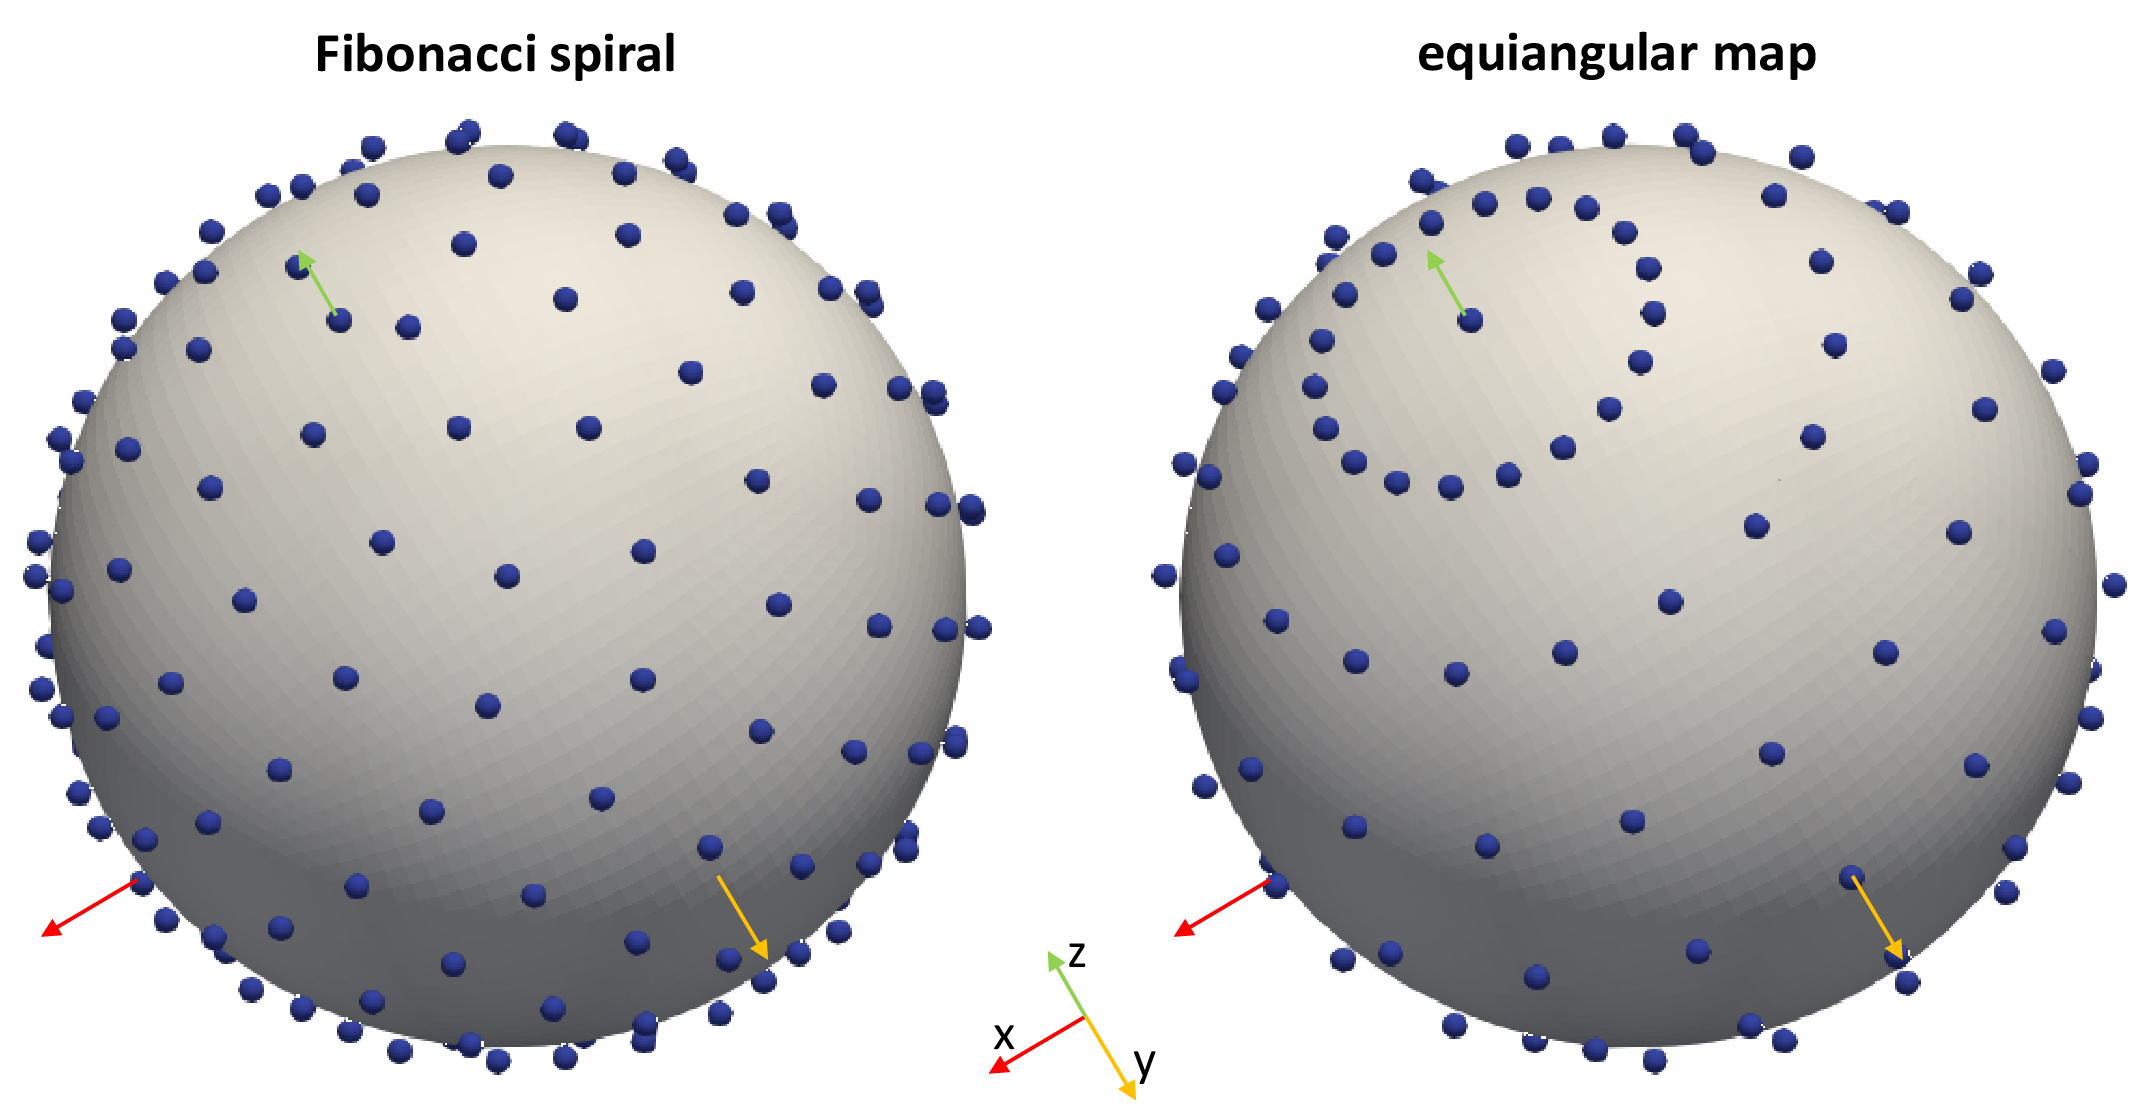
\includegraphics[scale=0.75]{../../benchmarks/gravity_prem/doc/spiral_VS_map_sampling.jpg}
\caption{Fibonacci spiral vs. equiangular map sampling scheme. The gray sphere represents the Earth and the blue dots are the measurement points located 225\si{km} above the Earth surface. Both sampling schemes create 200 points in this example.}
\label{fig:gravityspiral}
\end{figure}

Two python scripts are also included along side input files to transform the generated ascii files into vtu:
{\sl gravity\_ascii\_to\_vtu\_map.py} which generates a latitude-longitude map view of the results contained in the ascii file, and {\sl gravity\_ascii\_to\_vtu\_sphere.py}
which generates a 3D point-wise vtu file of the gravity vector and potential.


%-----------------------------------------------------------------------
\paragraph{Benchmark~1: hollow sphere with constant density}
\hfill \break
The corresponding input file is \texttt{gravity\_constant\_density.prm}.
This input file generates a hollow sphere mesh geometry filled with a single material of constant density.  

A custom mesh is generated with a higher resolution towards the surface. Its inner radius is $R_1=3481 \si{km}$ and its outer radius is $R_2=6371 \si{km}$. The mesh is specified as follows in the prm file:

\begin{lstlisting}
subsection Geometry model
  set Model name = spherical shell
  subsection Spherical shell
    set Inner radius  = 3481000
    set Outer radius  = 6371000
    set Opening angle = 360
    set Custom mesh subdivision = list of radial values
    set List of radial values = 5000000, 6000000, 6300000, 6366000
    set Initial lateral refinement = 4
  end
end
\end{lstlisting}

A surface mesh at the outer radius is first generated and refined as desired according to the initial lateral refinement (here set at 4), before it is extruded radially. One must then specify the subdivision method that is employed to create a custom mesh. A list of radial values subdivides the spherical shell at specified radii (in addition to the inner radius), here at 5000, 6000, 6300 and 6366 \si{km}. The mesh may be globally refined afterwards in the subsection mesh refinement.

\begin{figure}[h!]
\centering
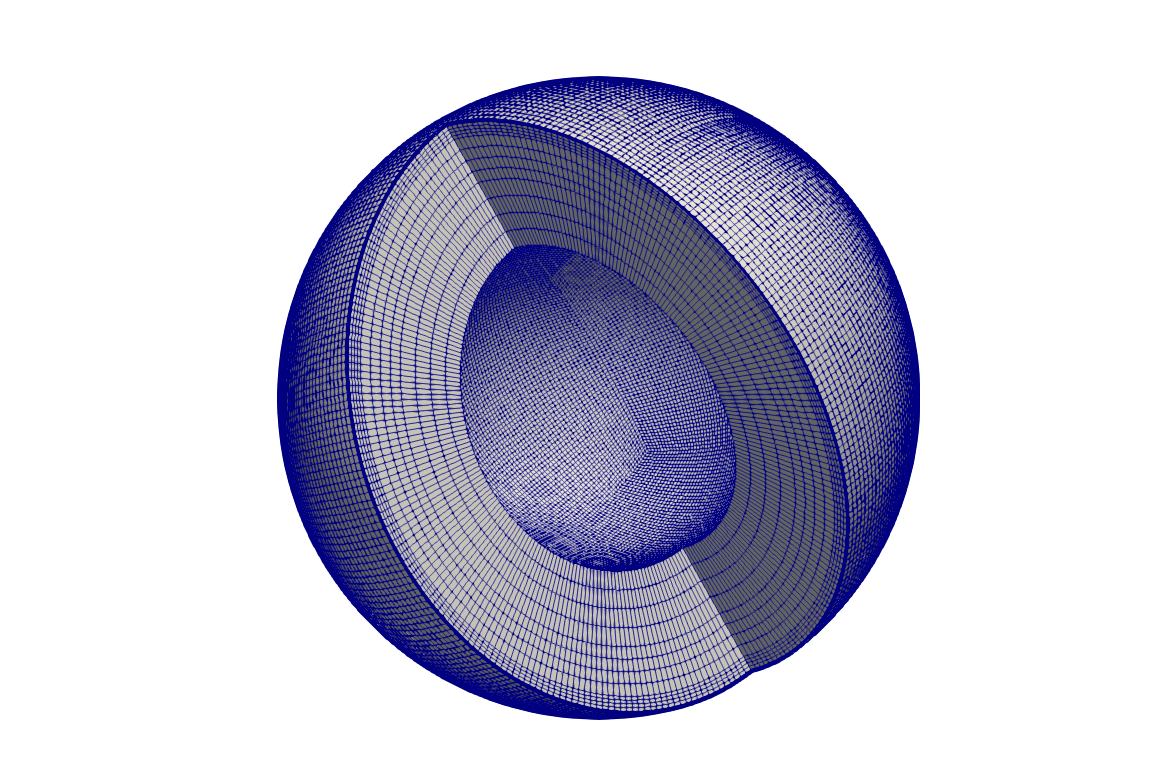
\includegraphics[width=0.48\linewidth]{../../benchmarks/gravity_prem/doc/custom_shell_full.png}
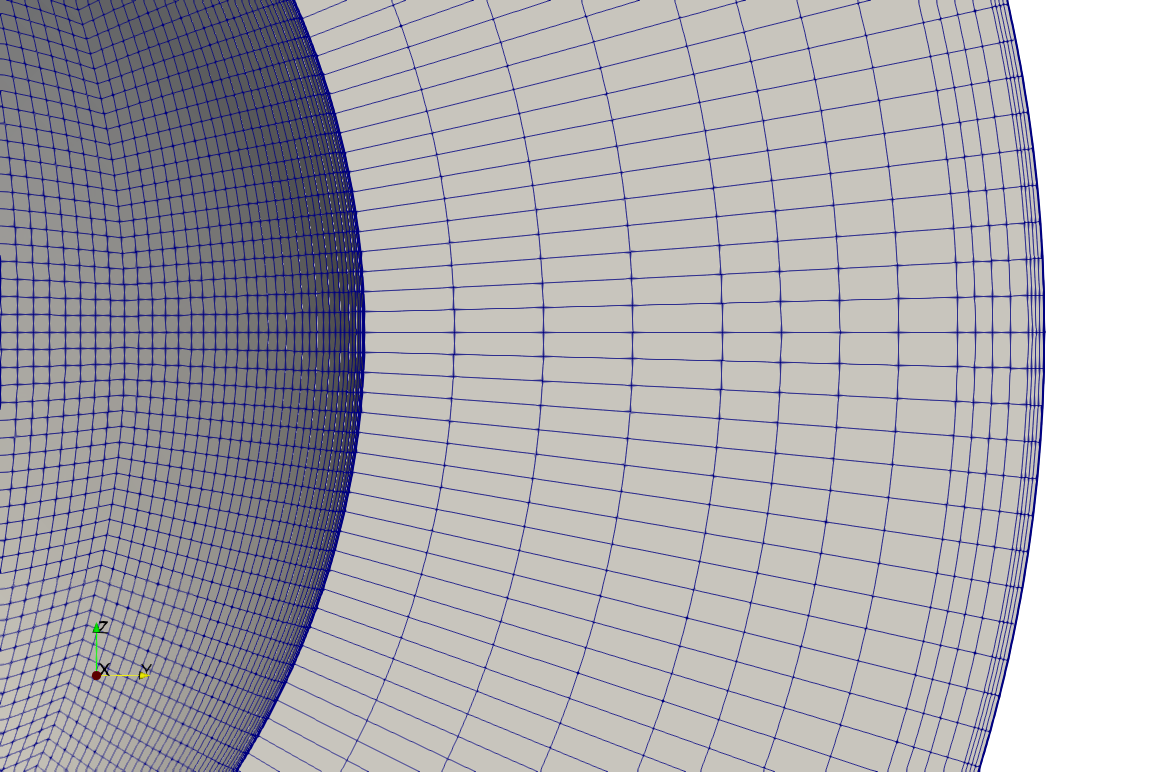
\includegraphics[width=0.48\linewidth]{../../benchmarks/gravity_prem/doc/custom_shell_zoom.png}
\caption{Hollow sphere mesh using the custom spherical mesh method. The surface mesh is first generated with an initial mesh refinement (here 4). Then the surface mesh is extruded radially and subdivided at the specified radii (here 5000, 6000, 6300 and 6366 \si{km}) before it is globally refined as desired (here by two levels of refinement). This produces a hollow sphere of 61440 elements.}
\label{fig:gravityline}
\end{figure}

The gravity potential $U$ is solution to the Poisson equation 
${\mathbf \nabla}^2 U = 4\pi {\cal G} \rho$ \cite{TS14}, where ${\cal G}$ is the gravitational constant.
In this first benchmark the density is constant and equal to $\rho_0$ for $R_1\leq r \leq R_2$, which allows us to compute an analytical solution as described below.
Outside the spherical shell the Poisson equation then becomes the Laplace equation $\Delta U=0$, which in spherical coordinates simplifies to: 
\begin{equation}
\frac{1}{r^2} \frac{\partial }{\partial r} \left(r^2 \frac{\partial U}{\partial r} \right) = 0 
\end{equation}
because of the symmetry of the problem. It has the simple solution:
\begin{equation}
g=\frac{\partial U}{\partial r} = \frac{C}{r^2} \label{eq:app1}
\end{equation}
where $C$ is a constant.
In order to avoid an infinite gravity field at $r=0$ (where the density is also zero), we need to impose $C=0$, i.e. the 
gravity is zero for $r<=R_1$.
Inside the shell, $\rho=\rho_0$ and we easily obtain:
\begin{equation}
g=\frac{\partial U}{\partial r} = \frac{4 \pi}{3} {\cal G} \rho_0 r + \frac{A}{r^2}
\end{equation}
where $A$ is an integration constant. 
We know that $g=0$ at the inner boundary $r=R_1$ so we can easily compute $A$ to obtain:
\begin{equation}
g=\frac{\partial U}{\partial r} = \frac{4 \pi}{3} {\cal G} \rho_0 (r - \frac{R_1^3}{r^2}). \label{eqgin}
\end{equation}
The branch for $r\geq R_2$ is given by Eq. (\ref{eq:app1}) and requiring the gravity field to be continuous at $r=R_2$:
\begin{equation}
g(r) = \frac{{\cal G} M}{r^2} \label{eqgout}
\end{equation}
where $M=\frac{4\pi}{3}\pi\rho_0(R_2^3-R_1^3)$ is the mass contained in the shell.
Turning to the potential, we obtain its expression for $r>=R_2$ by integrating Eq.(\ref{eqgout}):
\begin{equation}
U(r)=-\frac{{\cal G}M}{r} +D
\end{equation}
where $D$ is an integration constant which has to be zero since we require the potential to vanish for $r\rightarrow \infty$.
For $R_1\leq r \leq R_2$, Eq. (\ref{eqgin}) yields:
\begin{equation}
U(r)= \frac{4 \pi}{3} {\cal G} \rho_0 \left(\frac{r^2}{2} + \frac{R_1^3}{r} \right)  + E 
\end{equation}
where $E$ is a constant. Continuity of the potential at $r=R_2$ requires that
\begin{equation}
E=-2\pi\rho_0 {\cal G}R_2^2.
\end{equation}
Since gravity is zero for $r\leq R_1$ the potential is constant there and a continuity requirement yields
\begin{equation}
U(r)=2\pi {\cal G}\rho_0 (R_1^2-R_2^2).
\end{equation}

We first start computing the gravity field and potential on a line 
of 15000 \si{km} length starting in the center of the Earth and passing through the (arbitrary) coordinates of 115\si{\degree} longitude and 87\si{\degree} latitude (so as to avoid cancelling effects due to symmetry), comprising 151 number of equidistant measurement points.
This translates as follows in the prm file:
\begin{lstlisting}
subsection Postprocess
  set List of postprocessors = gravity calculation
  subsection Gravity calculation
    set Sampling scheme             = map
    # Specify the longitude coordinate of the profile
    set Number points longitude     = 1
    set Minimum longitude           = 115
    set Maximum longitude           = 115
    # Specify the latitude coordinate of the profile
    set Number points latitude      = 1
    set Minimum latitude            = 87
    set Maximum latitude            = 87
    # Specify the number of point along the profile and 
    # its length between minimum and maximum radius
    set Number points radius        = 151
    set Minimum radius              = 0
    set Maximum radius              = 15000000
  end
end
\end{lstlisting}

The sampling scheme is a map with only a single point in longitude and a single point in latitude, but 151 points in radius. To set the location of the longitude and latitude point where the radial line passes through the surface, we specify the minimum longitude (115\si{\degree}) and minimum latitude (87\si{\degree}). Setting a maximum longitude/latitude is not required because only one point is set, and the sampling always starts from the minimum longitude/latitude. Along the radial line, the 151 points are scattered equally from the minimum radius 0 \si{km} to maximum radius 15000 \si{km}, which results in sampling every 100 \si{km} along the profile. Results are shown in Fig.~\ref{fig:gravityline} and match the analytical solution presented above. 

Gravity can also be measured at a set of desired locations in space. We have chosen 10 points at an altitude of 225 \si{km} corresponding to the 10 cities listed in Table~\ref{tab:cities}. Listing a single value for a radius will be interpreted as all points sharing the same altitude/radius. This translates as follows into the prm file:

\begin{lstlisting}
subsection Postprocess
  set List of postprocessors = gravity calculation
  subsection Gravity calculation
    set Sampling scheme             = list of points 
    set List of radius              = 6596000
    set List of longitude           = 38.7578, 174.7633, -157.8583,   85.324, -77.0428,   2.3522, -21.9426, -122.4194, 139.6917,  16.3738
    set List of latitude            =  8.9806, -36.8485,   21.3069,  27.7172, -12.0464,  48.8566,  64.1466,   37.7749,  35.6895,  48.2082 
  end
end
\end{lstlisting}

Results are shown in Fig.~\ref{fig:gravitycities}. Measurements agree well with the expected analytical value. The remaining anomalies are consequence of the mesh resolution and the quadrature order, and disappear with higher resolution.
  
\begin{table}
\centering
\begin{tabular}{llll}
\hline
Index & City & Latitute & Longitude \\
\hline\hline
 0 & Addis Ababa &8.9806\si{\degree}N & 38.7578\si{\degree}E \\
 1 & Auckland & 36.8485\si{\degree}S & 174.7633\si{\degree}E \\
 2 & Honolulu &21.3069\si{\degree}N & 157.8583\si{\degree}W \\
 3 & Kathmandu &27.7172\si{\degree}N & 85.3240\si{\degree}E \\
 4 & Lima &12.0464\si{\degree}S & 77.0428\si{\degree}W \\
 5 & Paris & 48.8566\si{\degree}N & 2.3522\si{\degree}E \\
 6 & Reykjavik & 64.1466\si{\degree}N & 21.9426\si{\degree}W \\
 7 & San Francisco & 37.7749\si{\degree}N & 122.4194\si{\degree}W \\ 
 8 & Tokyo & 35.6895\si{\degree}N & 139.6917\si{\degree}E \\
 9 & Vienna &48.2082\si{\degree}N & 16.3738\si{\degree}E \\
\hline
\end{tabular}
\caption{List of the 10 implemented cities and their latitude/longitude coordinates.}
\label{tab:cities}
\end{table}

\begin{figure}[h!]
\centering
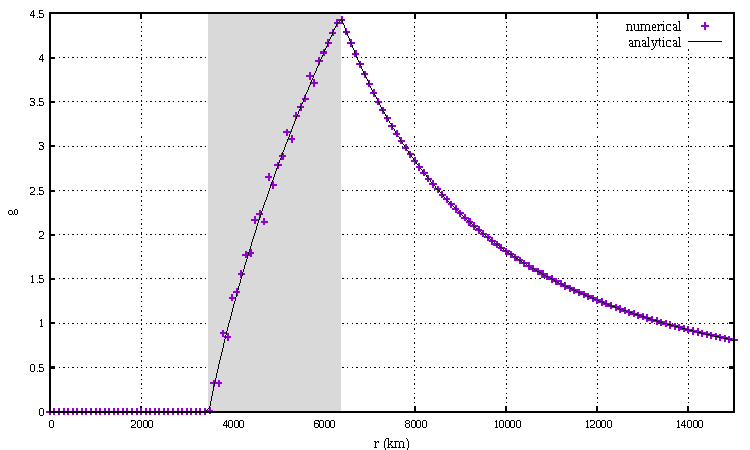
\includegraphics[width=0.48\linewidth]{../../benchmarks/gravity_prem/doc/profile_gravity_const_g.pdf}
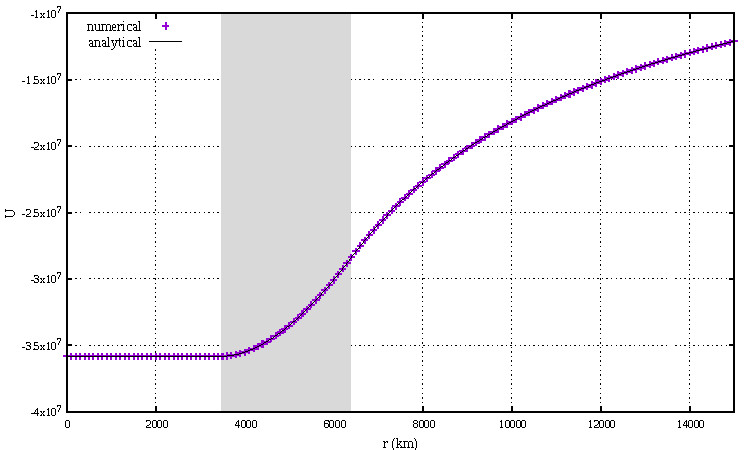
\includegraphics[width=0.48\linewidth]{../../benchmarks/gravity_prem/doc/profile_gravity_const_U.pdf}
\caption{Gravity acceleration $|{\mathbf g}|$ and potential $U$ along a radial profile for a hollow sphere of constant density of 3000 \si{\kilogram\per\cubic\metre}. The grey area symbolises the hollow sphere interior where density is non zero. The analytical solution is also shown in black.}
\label{fig:gravityline}
\end{figure}

 \begin{figure}[h!]
\centering
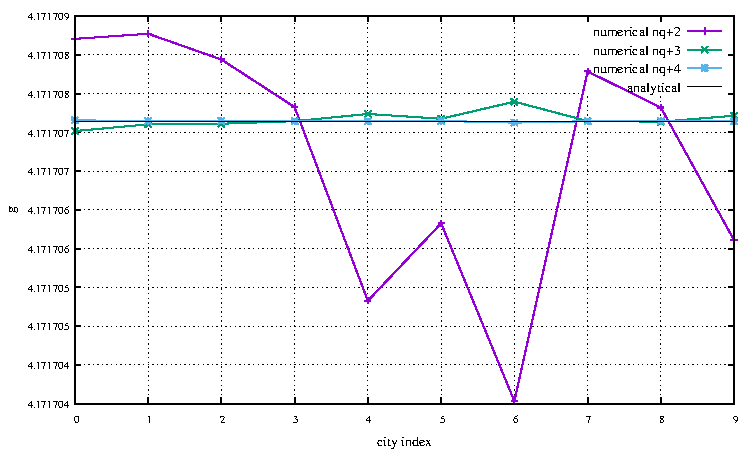
\includegraphics[width=0.48\linewidth]{../../benchmarks/gravity_prem/doc/cities_gravity_const_g.pdf}
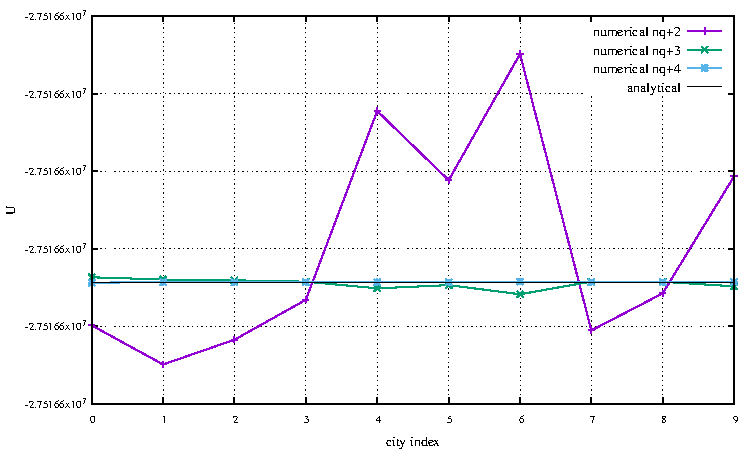
\includegraphics[width=0.48\linewidth]{../../benchmarks/gravity_prem/doc/cities_gravity_const_U.pdf}
\caption{Gravity acceleration $|{\mathbf g}|$ and potential $U$ at GOCE height  (225 \si{km}) above 10 cities measurement points for a hollow sphere of constant density of 3000 \si{\kilogram\per\cubic\metre} counting 61440 elements. We varied the increased quadrature point degree from 2 to 4 to illustrate the rapid convergence of the gravity and potential toward the analytical solution shown in black.}
\label{fig:gravitycities}
\end{figure}

%-----------------------------------------------------------------------------
\paragraph{Benchmark~2: full sphere with PREM density}
\hfill \break
The corresponding input file is \texttt{gravity\_PREM\_density.prm}.
This input file generates a full sphere and assigns a density field based on the PREM values, as shown in Fig.~\ref{fig:gravitywholesphere}.

A new material model is provided for this benchmark in the {\sl prem.cc} file, which implements the radial density as obtained from original publication of the PREM model \cite{dzan81} and reproduced in Table~\ref{tab:premdensity}.

\begin{table}
\centering
\begin{tabular}{lll}
\hline
inner core & $0<r<1221.5$\si{km} & $\rho(x) =13.0885-8.8381 x^2$ \\
outer core & $1221.5<r<3480$\si{km} & $\rho(x)=12.5815-1.2638x-3.6426x^2-5.5281x^3$\\
Lower mantle &$3480<r<5701$\si{km} & $\rho(x)=7.9565-6.4761x+5.5283x^2-3.0807x^3$\\
transition zone 1 & $5701<r<5771$\si{km} & $\rho(r)=5.3197-1.4836x$\\
transition zone 2 & $5771<r<5971$\si{km} & $\rho(r)=11.2494-8.0298x$\\
transition zone 3 & $5971<r<6151$\si{km} & $\rho(r)=7.1089-3.8045x$\\
Low velocity zone &$6151<r<6291$\si{km} & $\rho(r)=2.6910+0.6924x$\\
LID  &$6291<r<6346.6$\si{km} & $\rho(r)=2.6910+0.6924x$\\
Lower Crust &$6346.6<r<6356$\si{km} & $\rho(r)=2.9$\\
Upper Crust &$6356<r<6368$\si{km} & $\rho(r)=2.6$\\
Ocean &$6368<r<6371$\si{km} & $\rho(r)=1.020$\\
\hline
\end{tabular}
\caption{List of ten layers defining the PREM model and their corresponding polynomial expression for the density as a function of $x=r/R_{Earth}$.
Note that the returned densities should be multiplied by 1000 to obtain
units of \si{\kilogram\per\cubic\metre}.}
\label{tab:premdensity}
\end{table}

As in the first benchmark, gravity is computed on a line and results are shown in Fig.~\ref{fig:gravityline2}. The PREM publication also specifies the gravity inside the planet and we show that the benchmark results agree with the published PREM profile. Also, we recover a value of 9.81 \si{\metre\per\square\second} at the surface of the Earth as expected. 

\begin{figure}[h!]
\centering
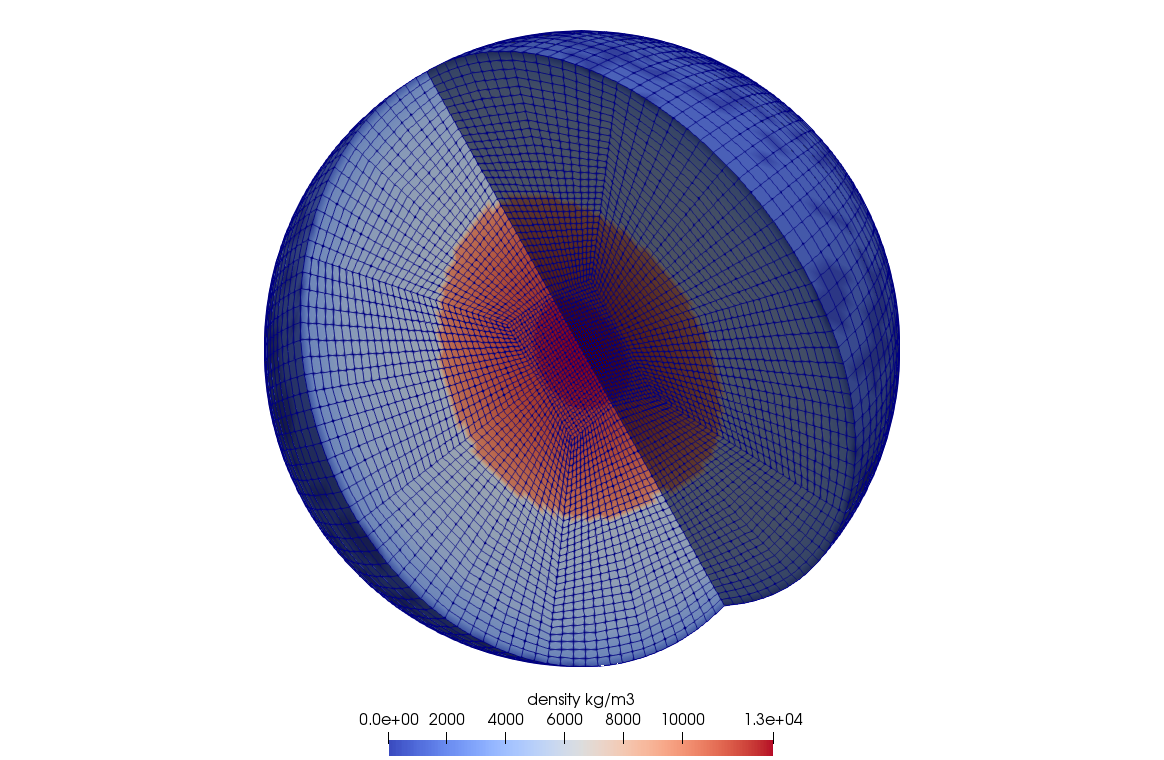
\includegraphics[scale=0.30]{../../benchmarks/gravity_prem/doc/default_shell_full.png}
\caption{Full spherical mesh generated using the default mesh generation method. The sphere counts 28672 elements and its density is defined using the PREM densities.}
\label{fig:gravitywholesphere}
\end{figure}

\begin{figure}[h!]
\centering
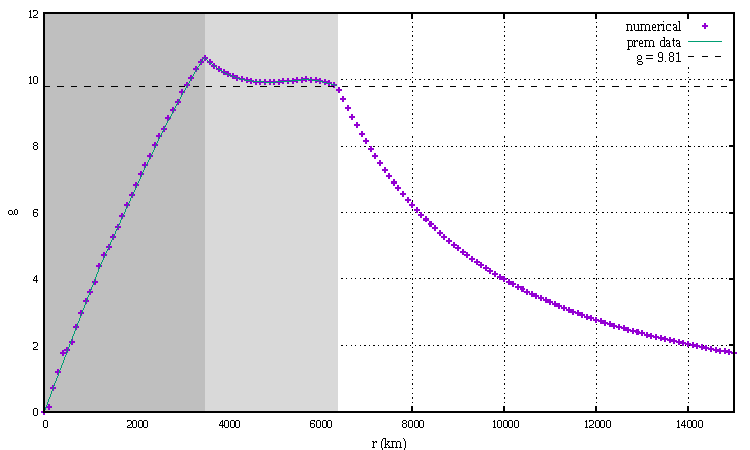
\includegraphics[width=0.48\linewidth]{../../benchmarks/gravity_prem/doc/profile_gravity_prem_g.pdf}
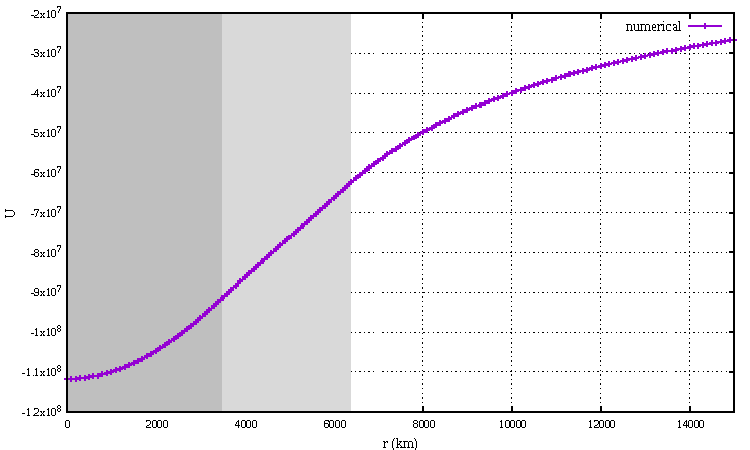
\includegraphics[width=0.48\linewidth]{../../benchmarks/gravity_prem/doc/profile_gravity_prem_U.pdf}
\caption{Gravity acceleration $|{\mathbf g}|$ and potential $U$ along a radial profile for a sphere of PREM density. The dark grey area specifies the core of Earth and the light grey area represents the mantle and crust of Earth. The PREM data gravity acceleration is also shown in green, as well as the average gravity of 9.81 \si{\metre\per\square\second} at the Earth surface.}
\label{fig:gravityline2}
\end{figure}

Gravity can be computed on a set of regularly spaced points in the latitude-longitude space. The sampling scheme is a map at GOCE height (altitude of 225 \si{km}): we only set the minimum radius at 6371+225=6596 \si{km} and 1 number points radius. To get a map of the whole Earth, we set the number of points longitude and latitude 73 and 37, respectively, which represents a field of points scattered every 5\si{\degree}. Here we do not need to specify a minimum and maximum longitude and latitude as their default are -180\si{\degree} to -180\si{\degree} and -90\si{\degree} to 90\si{\degree}, respectively:
\begin{lstlisting}
subsection Postprocess
  set List of postprocessors = gravity calculation   
  subsection Gravity calculation
    set Sampling scheme             = map
    set Minimum radius              = 6596000
    set Number points radius        = 1
    set Number points longitude     = 73
    set Number points latitude      = 37
  end
end
\end{lstlisting}

We used the python script provided with the benchmark to convert the output gravity file into a vtu file. This script converts the ascii output into a vtu file and allows us to plot the gravity acceleration, potential and gradients in ParaView, as shown in Fig.~\ref{fig:gravitymapfull} and Fig.~\ref{fig:gravitymapfull2}. 

\begin{figure}[h!]
\centering
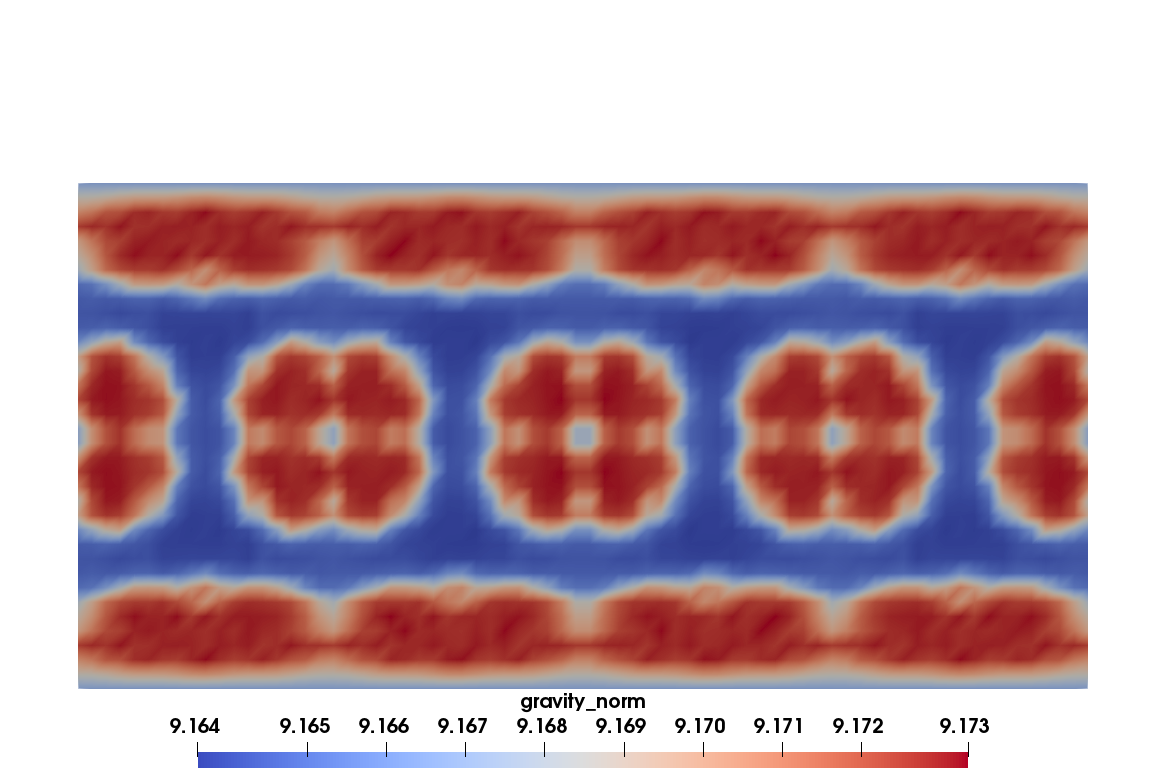
\includegraphics[width=0.48\linewidth]{../../benchmarks/gravity_prem/doc/prem_g_map.png}
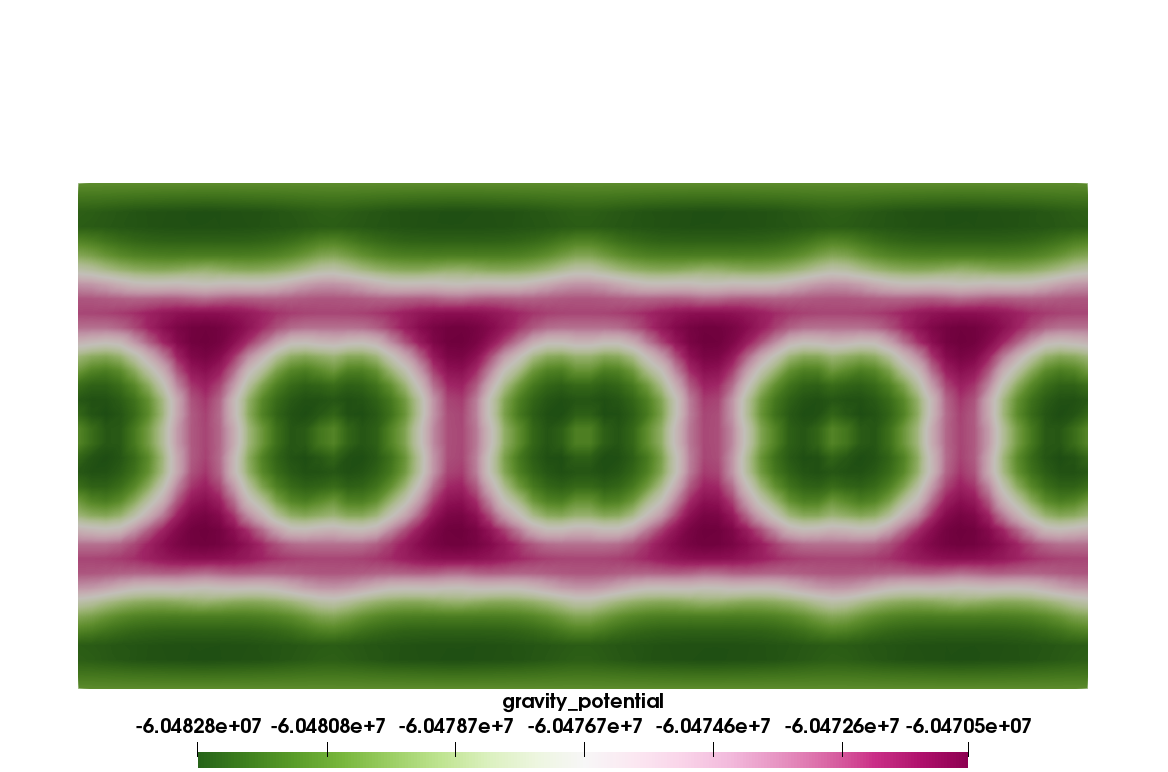
\includegraphics[width=0.48\linewidth]{../../benchmarks/gravity_prem/doc/prem_U_map.png}
\caption{Gravity acceleration $|{\mathbf g}|$ and potential $U$  for a sphere of PREM density at GOCE height.The patterns show the mesh build composed of 8 blocs.}
\label{fig:gravitymapfull}
\end{figure}

\begin{figure}[h!]
\centering
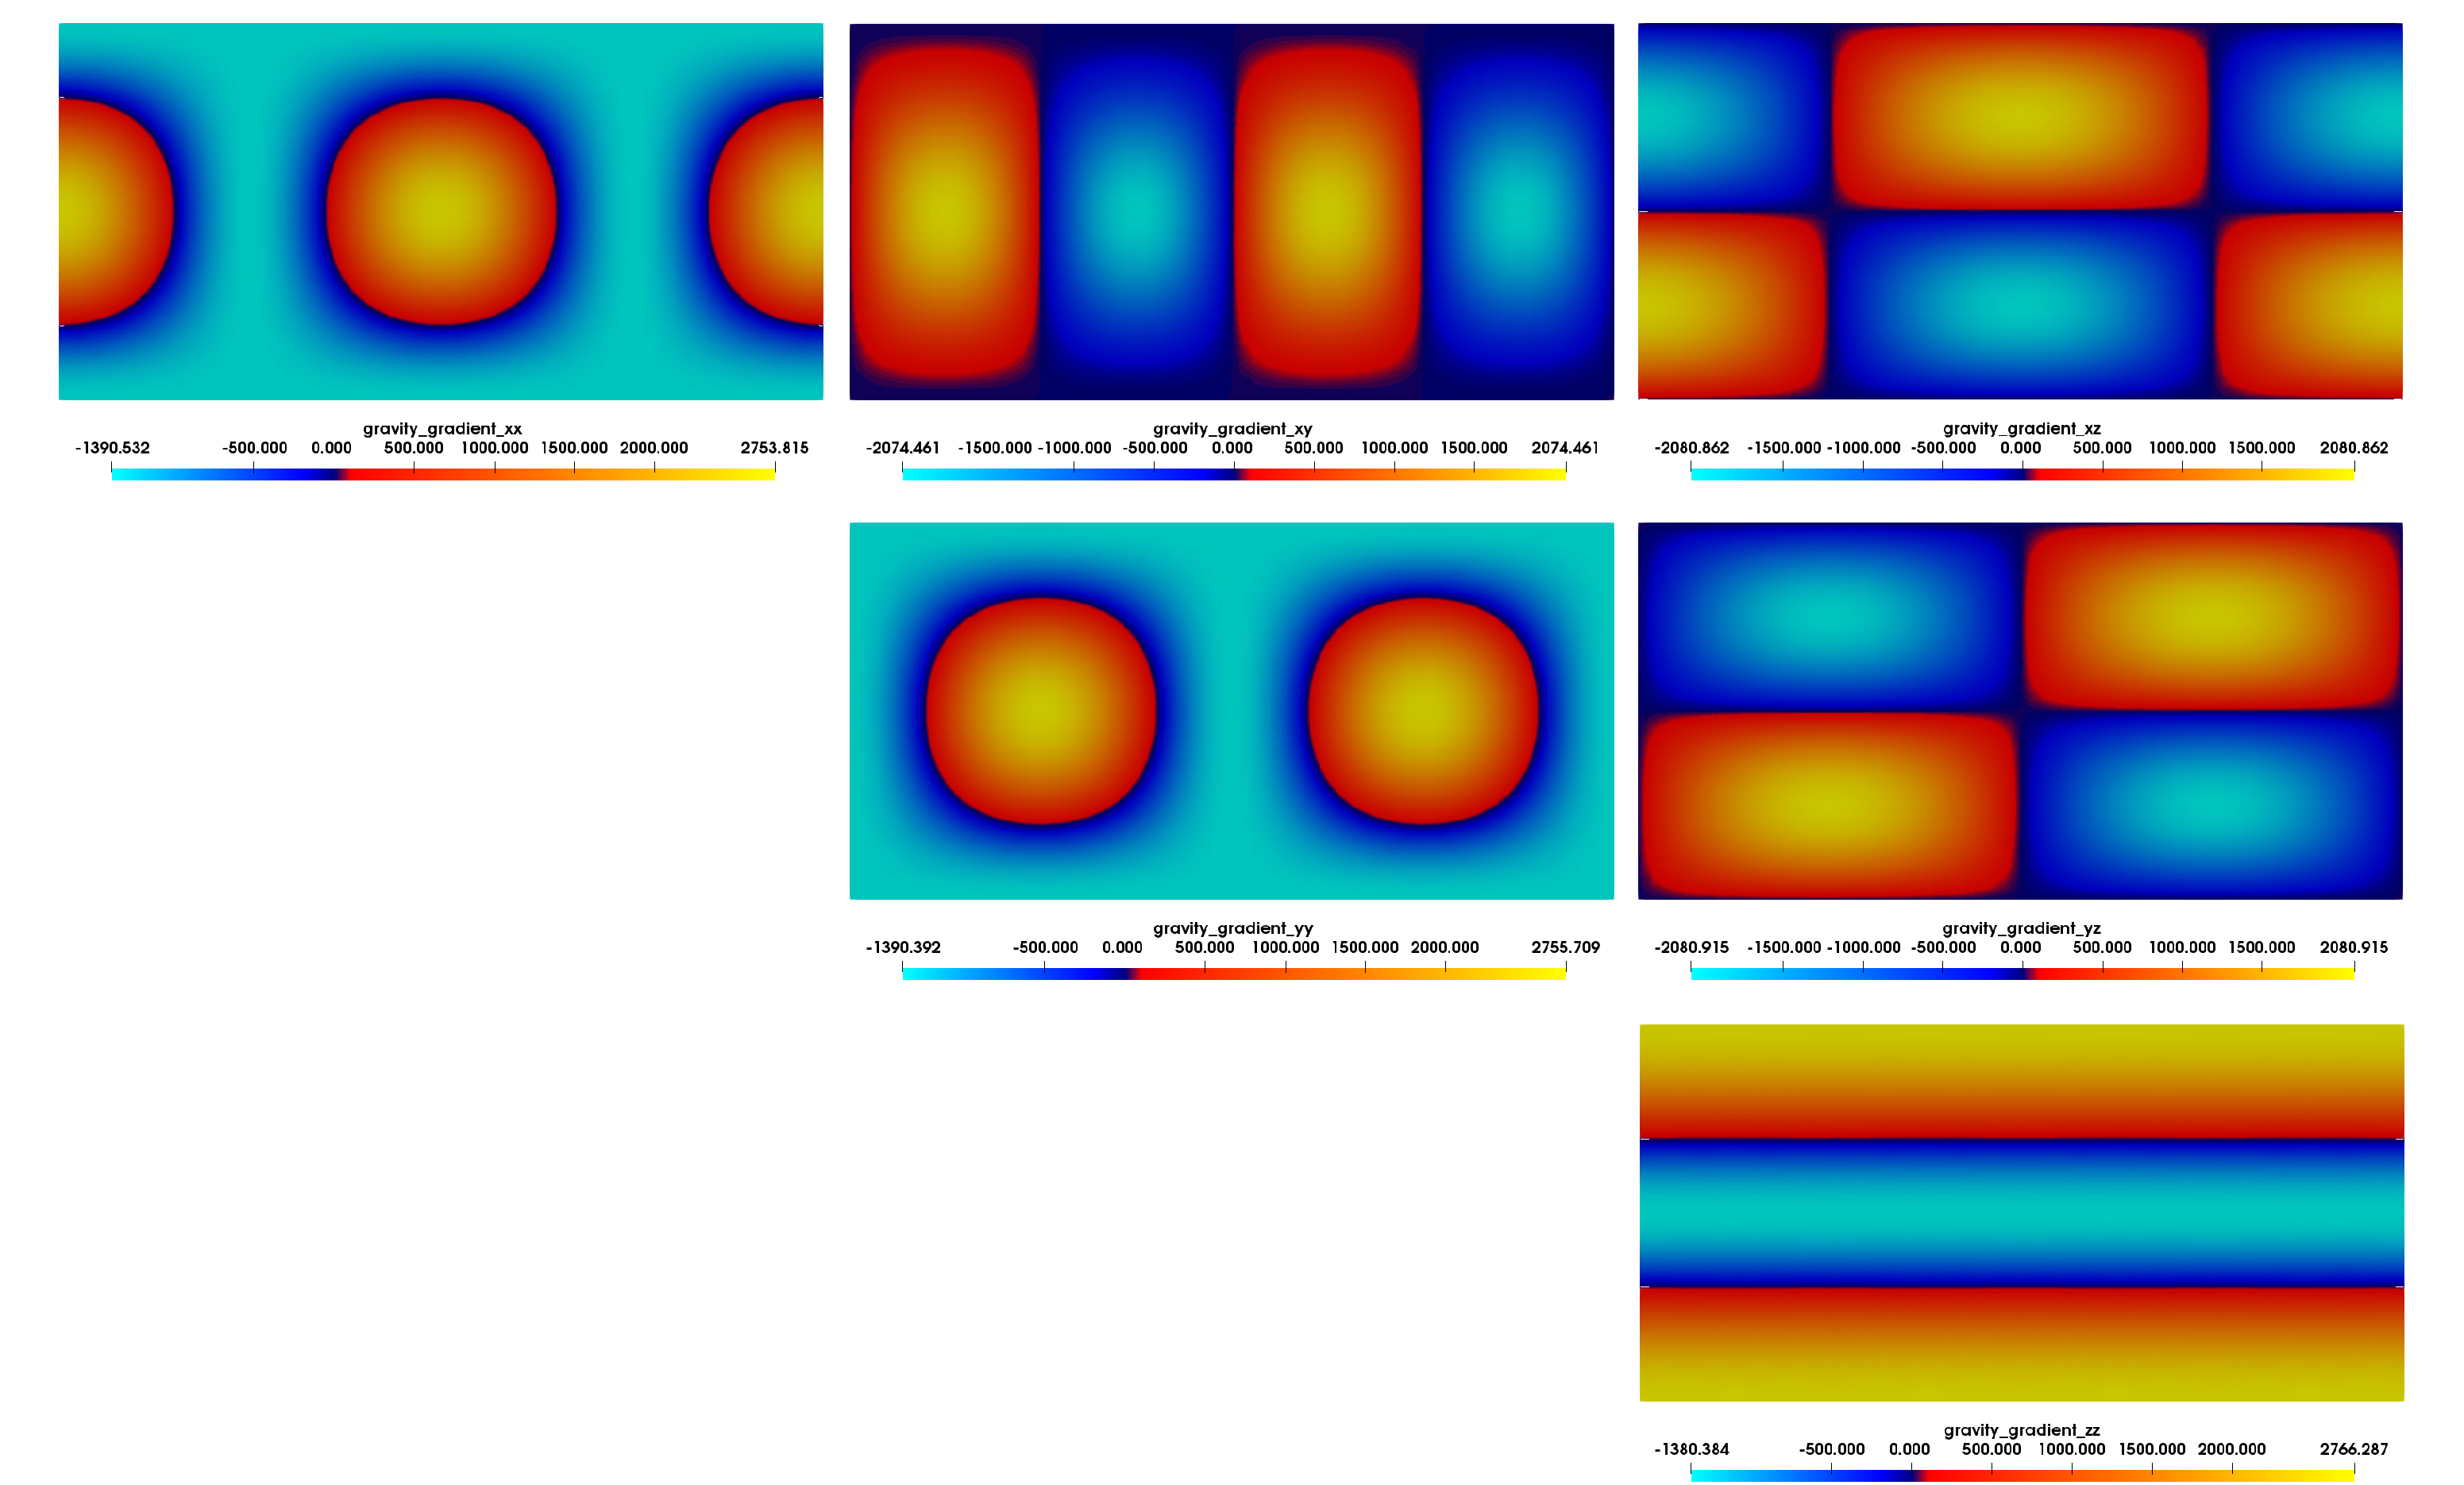
\includegraphics[scale=0.64]{../../benchmarks/gravity_prem/doc/gradient_prem_map.jpg}
\caption{Gravity gradients $g_{xx}$, $g_{xy}$, $g_{xz}$, $g_{yy}$, $g_{yz}$ and $g_{zz}$. Because of symmetry we do not show $g_{yx}$, $g_{zx}$ and $g_{zy}$. We purposefully choose this somewhat unusual color scale and center it on zero. Blue colors indicate negative values while red colors indicate positive value, with a sharp transition between both.}
\label{fig:gravitymapfull2}
\end{figure}

Gravity can also be computed on a Fibonacci spiral of points distributed around the planet, for instance at GOCE height. Here we use 2701 points to compare the results with the regularly spaced points map (37x73=2701). This translates as follows in the prm file:

\begin{lstlisting}
subsection Postprocess
  set List of postprocessors = gravity calculation
  subsection Gravity calculation
    set Sampling scheme               = fibonacci spiral
    set Number point fibonacci spiral = 2701
    set Minimum radius                = 6596000 
    set Number points radius          = 1
  end
end
\end{lstlisting}

Note that sampling becomes more uniform with increasing number point fibonacci spiral.

\begin{figure}[h!]
\centering
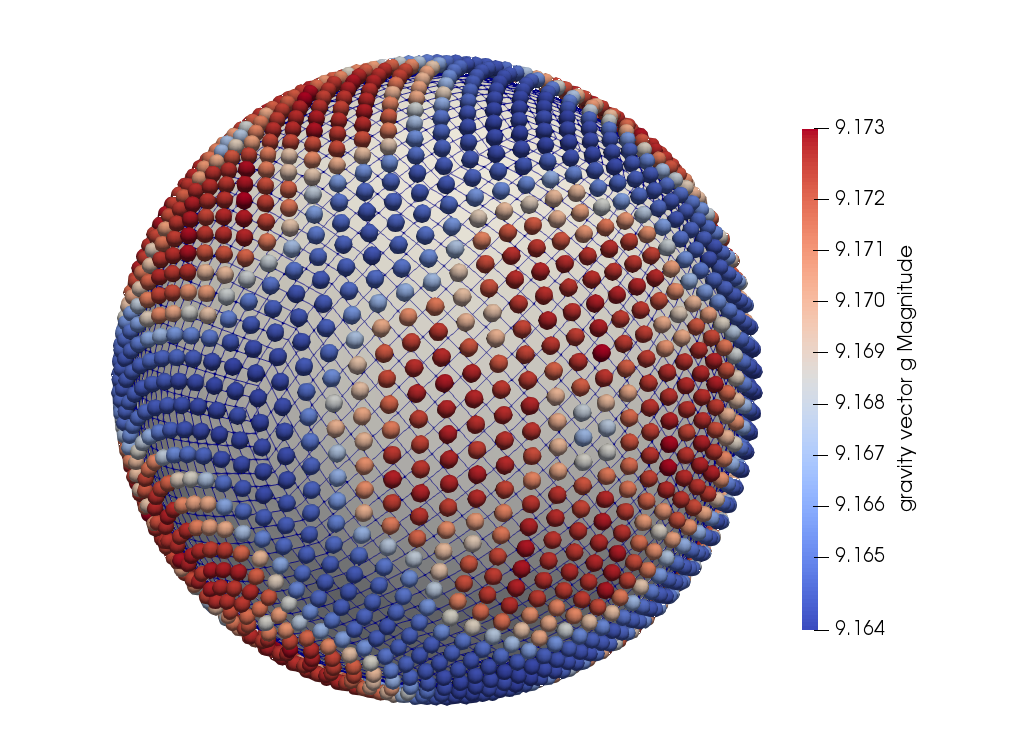
\includegraphics[scale=.4]{../../benchmarks/gravity_prem/doc/spiral_prem.png}
\caption{Gravity acceleration $|{\mathbf g}|$ at GOCE height using the Fibonacci spiral sampling scheme with 2701 measurement points.}
\label{fig:gravitypremspirals}
\end{figure}

\begin{figure}[h!]
\centering
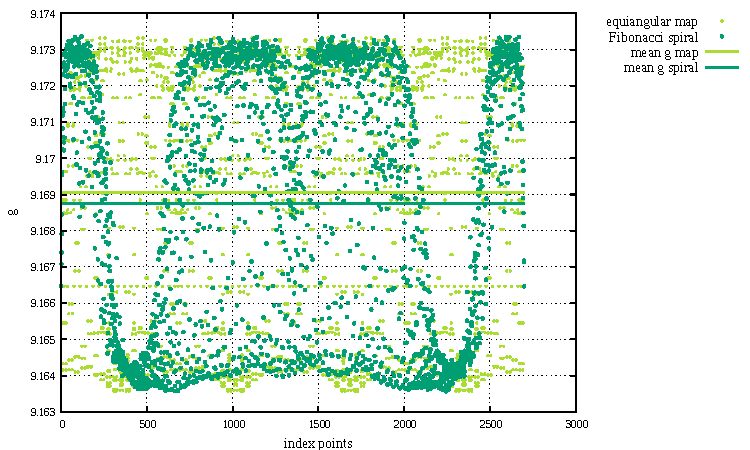
\includegraphics[scale=1.1]{../../benchmarks/gravity_prem/doc/stats_gravity_prem_g.pdf}
\caption{Gravity acceleration $|{\mathbf g}|$ for the equiangular map and Fibonacci spiral sampling scheme, and their respective gravity average. The average gravity is ~9.1 because it is calculated at GOCE height 225 km above the Earth surface.}
\label{fig:gravityprem}
\end{figure}
